\documentclass[a4paper,times,hidelinks,12pt]{article}
%\usepackage{indentfirst}
\usepackage{amsmath}
\usepackage{multirow}
\usepackage{graphicx}
\usepackage{float}
\usepackage{setspace}
\usepackage[bottom]{footmisc}
%\usepackage{svg}
\usepackage{subcaption}
%\usepackage{minted}
\onehalfspacing
\usepackage[top=2.5 cm, bottom=2.5 cm, left=4 cm, right=2.5 cm]{geometry}
\usepackage{hyperref}
\usepackage{algorithm}
\usepackage{rotating}
\usepackage[noend]{algpseudocode}

\makeatletter
\def\BState{\State\hskip-\ALG@thistlm}
\makeatother

\newcommand\tab[1][0.5cm]{\hspace*{#1}}
\newcommand*\dif{\mathop{}\!\mathrm{d}}

\setlength\parindent{0pt}

\begin{document}

\begin{titlepage}
\begin{center}
\vspace*{1cm}
\underline{\textbf{\Large ISTANBUL TECHNICAL UNIVERSITY}} \\[10 pt]

\underline{\textbf{\large FACULTY OF SCIENCE AND LETTERS}} \\[15 pt]

\textbf{\large Graduation Project} \\
\vspace{1.8 cm}

\includegraphics[scale=1.2]{itu_logo.pdf} \\
\vspace{1.8 cm}
%\textbf{\large Machine Learning and Nonlinear Schr{\"o}dinger Equation} \\[5 pt]
\textbf{\large Machine Learning and Non-linear Schr{\"o}dinger Equation} \\[5 pt]
\textbf{H{\"u}seyin Talha \c{S}enya\c{s}a}\\
\vspace{1.5 cm}
\end{center}
\vfill
\textbf{{Department : Physics Engineering}}\\
    \textbf{Student ID \hspace{0.2 cm}: 090120132}\\
    \textbf{Advisor\hspace{1.1 cm}: Assoc. Prof. A. Levent Suba\c{s}{\i}}
\vspace{2 cm}

\center\textbf{FALL 2017}

\end{titlepage}


%\title{\textbf{TEST}}
%\date{}
%\maketitle
\setcounter{page}{1}
\pagenumbering{roman}

\section*{Summary}

We train an artificial neural network to estimate the ground state energy
of a one-dimensional Bose-Einstein condensate in different type of potentials including random.
Such a system can be described by the solution of a non-linear Schr{\"o}dinger equation also called a Gross-Pitaevskii equation. We also use the method for the inverse problem of predicting the non-linearity parameter using the ground
state density profile for a given harmonic trapping potential.

\newpage
\tableofcontents

\newpage

\pagenumbering{arabic}
\section{Introduction and Motivation}


\label{sec:Intro}
%\noindent Machine learning.\\
%General usage area.\\
%ML in physics and Phyiscs in ML.\\
%ML\&SE article.\\
%Ours difference.\\



In quantum mechanical systems one must obtain the wave function to determine physical properties of the system. For single particle systems, obtaining the wave function is easy compared to many body systems. The solution can be even harder if the described system involves interaction between particles because such differential equations may have nonlinear terms. In nonlinear case, there are no general rule to solve and they are treated individually in most cases. If there are no analytic solution exists and approximation is not on the table then the only chance is numerical solution of the equation to obtain the wave function, and then one can determine the physical properties of the system. However, machine learning applications in recent years showed that physical properties of the system can be predicted without solving these equations. \\

The reason why machine learning has such a capability is that artificial neural networks used in machine learning can approximate any continuous function within desired accuracy. This means that if we take $\epsilon > 0$ as desired accuracy,  $\boldsymbol{y} = \boldsymbol{f}(\boldsymbol{x})$ (bold means vector) output of the network and $\boldsymbol{g}(\boldsymbol{x})$ real value of the function, then it is guaranteed that there exists a network that satisfies the relation $|\boldsymbol{g}(\boldsymbol{x}) - \boldsymbol{f}(\boldsymbol{x})| < \epsilon $. From this point of view, a process or calculation that can be thought of as a function can be represented by a corresponding neural network that mimics this function in desired accuracy \cite{nielsen2015neural}. With this in mind, neural networks have the potential to learn general functions and be exploited for their advantages. Approximate value of the quantity can be determined for different scenarios. \\

Many different kind of applications of machine learning have already been implemented in physics\footnote{For a detailed list, see \cite{physicsml}}. For example, In \cite{carleo2017solving, cai2017approximating} machine learning is applied to quantum many body problems. A machine learning method called Unsupervised Learning to detect patterns in big datasets is used for discovering phase transitions \cite{wang2016discovering}. There are also developed techniques in machine learning inspired from physics such as quantum tensor networks \cite{stoudenmire2016supervised}. Relation between physics and machine learning also caused foundation of a new branch called Quantum Machine Learning which aims to implement a quantum software to make machine learning faster than its classical version \cite{biamonte1611quantum}. \\

In \cite{mills2017deep}, machine learning approach is applied to a 2D Schr{\"o}dinger equation also known as Gross-Pitaevskii equation with random potentials. The authors built a convolutional deep neural network, and trained it to predict ground state energy of the system under four different confining potentials including random potential. Their study showed that machine learning is a promising alternative in electronic structure calculations of quantum systems. In our study inspired from the article mentioned above, we apply machine learning method to the nonlinear Schr{\"o}dinger equation to predict ground state energy of a Bose-Einstein condensate with random interaction parameter at absolute zero temperature under six different one dimensional trapping potentials including random. 


\section{Gross Pitaevskii Equation}

A Bose-Einstein Condensate (BEC) at zero temperature is described by Gross Pitaevskii equation (GPE) also known as non-linear Schrodinger Equation (NLSE). It is mean field approximation of a quantum many body system which the hamiltonian of the system is given by;

\begin{equation}
\label{eq:GPE_hamiltonian}
\hat{H} = \sum_{i = 1}^{N} \left(\frac{\boldsymbol{p}_i^2}{2m} + V(\boldsymbol{r}_i) \right) + \frac{1}{2} \sum_{i = 1}^{N} \sum_{j \neq i}^{N} U(|\boldsymbol{r}_i - \boldsymbol{r}_j|)
\end{equation}

where $\textbf{p}_i$ $i^{th}$ atom's momentum, $\boldsymbol{r}$ is position vector, $m$ is mass, $V$ is external potential and $U$ is interaction between $i^{th}$ and $j^{th}$  atoms. Since the ground state energy is the only possible minimum energy, one can minimize this hamiltonian in order to obtain ground state energy. To do that, the mean field approximation is utilized to represent all bosons with the same wave function since the condensate is at zero temperature which allows to assume that all bosons are at the ground state \cite{pethick2002bose}. The constraint in the minimization step involves satisfying the normalization condition that is given as,


\begin{equation}
\label{eq:GPE_normalization}
\int |\psi(\boldsymbol{r})|^2 \dif^3 \boldsymbol{r} = N    
\end{equation}

where $N$ is the number of particles in the system. This condition equals to minimizing the thermodynamic potential, free energy $F = E - \mu N$ such that $\delta F = 0 = \delta E - \mu \delta N = 0$ where $\mu$ is chemical potential \cite{pethick2002bose}. If we plug in the corresponding equations to this expression it becomes,  

\begin{equation}
\label{eq:GPE_derivation_free_energy}
F(\psi) = \int \psi^{*}\hat{H}\psi \dif^3\boldsymbol{r} - \mu \int |\psi|^2 \dif^3\boldsymbol{r}
\end{equation}

Therefore, the problem can be stated as minimization of the above equation \cite{rogel2013gross}. Applying variation method to this equation while treating $\psi^{*}$
and $\psi$ as independent objects and using $U(|\textbf{r}_i - \textbf{r}_j|) = g\delta(\textbf{r}_i - \textbf{r}_j)$ one can obtain Gross Pitaevskii Equation in stationary form as, 

\begin{equation}
\label{eq:GPE_time_indep}
\frac{-\hbar^2}{2m}\nabla^2\psi + V(\boldsymbol{r})\psi + g|\psi|^2\psi = \mu\psi
\end{equation}

%General form of GPE in three dimension is given as,
%
%\begin{equation}
%\label{eq:GPE_3D}
%i \hbar \frac {\partial \psi}{\partial t} = \frac {-\hbar^2}{2m}\nabla^2
%\psi + V(\boldsymbol{r}, t)\psi + g|\psi|^2\ \psi
%\end{equation}

\noindent where $\hbar$ is Planck constant, $\psi(\boldsymbol{r})$ is the wave function, $\nabla^2$ is the Laplacian operator, $g$ is interaction parameter and it is defined as 

\begin{equation}
\label{eq:GPE_inter_param}
g=\frac{4\pi\hbar^2a_s}{m}
\end{equation}

\noindent where, $a_s$ is the s wave scattering length. Nonlinearity of the equation is caused by the cubic term $g|\psi|^2$ which represents the interactions between bosons. The $|\psi|^2$ term is interpreted as density, thus; there occurs an energy contribution caused by the mean field interactions. If there is no interaction GPE reduces to the Schr{\"o}dinger Equation (SE) and becomes a linear equation. By definition, $g$ can be positive or negative. If $g > 0$, it represents repulsive interaction, and if $g < 0$, it represents attractive interactions \cite{barenghi2016primer}. The time evolution of the system must occur according to the Schr{\"o}dinger Equation, therefore; the time dependent GPE can be written as,

\begin{equation}
\label{eq:GPE_time_evolution}
i \hbar \frac{\partial\Psi(\boldsymbol{r}, t)}{\partial t} = \hat{H}\Psi(\boldsymbol{r}, t)
\end{equation}

where $t$ is time and $\Psi(\boldsymbol{r}, t) = \psi(\boldsymbol{r})e^{-i\mu t/\hbar} $. If it is rewritten in open form,

\begin{equation}
\label{eq:GPE_time_indep}
i \hbar \frac{\partial\Psi(\boldsymbol{r}, t)}{\partial t} = [\frac{-\hbar^2}{2m}\nabla^2 + V(\boldsymbol{r}) + g|\Psi(\boldsymbol{r}, t)|^2 ] \Psi(\boldsymbol{r}, t)
\end{equation}

The ground state energy of the system is given in Eq.~\eqref{eq:GPE_derivation_free_energy} which is,

\begin{equation}
\label{GPE_total_energy_general}
\langle E \rangle = \int \Psi^{*}\hat{H}\Psi \dif^3\boldsymbol{r}
\end{equation}

\begin{equation}
\label{GPE_total_energy}
E = \int \left(\frac {\hbar^2}{2m}|\nabla
\Psi|^2 + V|\Psi|^2 + \frac{g}{2}|\Psi|^4 \right) d^3\boldsymbol{r}
\end{equation}

Here, the terms represent kinetic, potential and interaction energy respectively.\footnote{Contribution from the interaction energy is divided by two to eliminate double counting while pairing bosons.} The potential does not depend on time so the hamiltonian does not too which means the total energy of the system is conversed. 

 
%\subsection{General information about GPE}
%\subsection{Why and how nonlinearty is introduced.}
%\subsection{Physical and mathematical interpretation of interaction parameter. (phy: attractive, %repulsive  math:dominance of the terms)}
%\subsection{Stationary form.}
%\subsection{Potential, kinetic and interaction energy expressions.}
\subsection{Reduction of dimension.}
\subsection{Analytic solution and approximation.}

There is no general solution for GPE and known analytic solutions exist only for few cases. In our study, infinite well and harmonic potential with zero interaction parameter has analytic solutions. The ground state energies are given by

\begin{equation}
\label{eq:GPE_1D_solution_harmonic}
    \mu = \frac{1}{2}\hbar\omega
\end{equation}


GPE generally solved by numerically or by approximation such as variational calculation or Thomas-Fermi approximation. \textbf{dilute}

\subsubsection{Thomas Fermi Approximation}



It is said that the second derivative term with respect to position represents the kinetic energy. When the potential and the interaction energy are dominant compared to the kinetic energy, the kinetic term can be neglected. This situation occurs when the condensate is large adequately and the interaction between bosons is repulsive \cite{pethick2002bose}. In another perspective, neglecting the kinetic term equivalent to making an assumption that there is no difference between the energy requirements to add a particle at arbitrary points \cite{rogel2013gross}. When the kinetic term is dropped, the new equation can be written as;

\begin{equation}
\label{eq:GPE_1D_thomas_fermi}
    V(x)\psi(x) + g|\psi(x)|^2\psi(x) = \mu\psi(x)
\end{equation}
this equation is analytically solvable and the solution is given by,


\begin{equation}
\label{eq:thomas_fermi_solution}    
n(x) = |\psi(x)|^2 =  
    \begin{cases}
        (\mu_{TF} - V)/g &\quad\text{if }  |x| \le x_{TF}  \\
        0 &\quad \textit{otherwise} \\
    \end{cases}
\end{equation}

where $x_{TF}$ is called Thomas-Fermi Length and $n(x)$ is density. The density defined in this range and cannot be negative, therefore; if the normalization condition Eq.~\eqref{eq:GPE_normalization} is applied then the equation reads,  

\begin{equation}
    \label{eq:thomas_fermi_mu_integral}
        \int_{-\infty}^{\infty} |\psi|^2 \dif x = \int_{-x_{TF}}^{x_{TF}} \frac{(\mu - V)}{g} \dif x = N 
    \end{equation}

With this equation, density of the system can be obtain via invoking boundary conditions. For an exact analytic expression example, one dimensional harmonic potential can be used, 

\begin{equation}
   \frac{1}{g} \left [ \int_{-x_{TF}}^{x_{TF}} \mu \dif x - \int_{-x_{TF}}^{x_{TF}} \frac{1}{2}m\omega^2x^2 \dif x \right ] = N
\end{equation}

\begin{equation}
\label{eq:thomas_fermi_integral_result}
    \frac{2\mu x_{TF}}{g} - \frac{m\omega^2 x_{TF}^3}{3g} = N
\end{equation}


From boundary conditions,
\begin{equation}
\label{eq:thomas_fermi_mu_bound}
    \mu = V(x_{TF}) = \frac{1}{2}m\omega^2x_{TF}^2    
\end{equation}


If we combine Eq.~\eqref{eq:thomas_fermi_integral_result} and Eq.~\eqref{eq:thomas_fermi_mu_bound} the equations reads,

\begin{equation}
    \frac{m\omega^2 x_{TF}^3}{g} - \frac{m\omega^2 x_{TF}^3}{3g} = N
\end{equation}


\begin{equation}
    \frac{4}{3} \left( \frac{2\mu}{m\omega^2} \right)^{1/2} \frac{\mu}{g} = N
\end{equation}

\begin{equation}
    \mu = \left(\frac{9}{32} (N\omega g)^2 m \right)^{1/3}
\end{equation}

Here we give comparison of densities obtained by numerical solution and Thomas-Fermi approximation for different potential types. 

\graphicspath{{"../figs/numericanalyze/"}}
\begin{figure}[H]
\centering
\begin{subfigure}[t]{0.45\textwidth}
    \includegraphics[width=\linewidth]{{{thomas-fermi-random-15.0}}}
\end{subfigure}
\begin{subfigure}[t]{0.45\textwidth}
    \includegraphics[width=\linewidth]{{{thomas-fermi-random2-15.0}}}
\end{subfigure}
\begin{subfigure}[t]{0.45\textwidth}
    \includegraphics[width=\linewidth]{{{thomas-fermi-random3-15.0}}}
\end{subfigure}
\begin{subfigure}[t]{0.45\textwidth}
    \includegraphics[width=\linewidth]{{{thomas-fermi-harmonic-gen}}}
\end{subfigure}
\caption{The upper left, right plots and the bottom left plot are random potentials with same interaction parameter. The bottom right is harmonic potential with different interaction parameters. The error between the numerical solution and approximation shrinks as the interaction parameter increases which corresponds to increment in interaction energy.}
\end{figure}



\subsection{Numerical Solution and Dataset Generation}

The dataset generation step is divided into two main parts and implemented independently. The first one is generating desired potential and the second one is numerical solution of the GPE under this potential by giving the generated potential to the numerical solution framework. The detailed description of the potential generation process is given in section~\ref{sec:potential_generation}. \\

In numerical solution part, we use a framework called XMDS \cite{dennis2013xmds2}, implemented specifically to solve differential equation systems with well optimized numerical methods. In this framework partial differential equation systems can be described by a markup language called XML.  When equation system is declared properly, XMDS produces a source code written in C++ that solves the equation with specified numerical method. Because of modularity in our implementation, the framework only solves the equation by supplied parameters, the framework does not generate anything internally such as potential, even the scaling factors are supplied externally. Such a modularity has an huge advantage such that changing numerical solution framework does not effect potential generation step, therefore; the work to change numerical solution framework is minimized. The only requirement is implementation of input output operations. By using this advantage, we also use another numerical solution framework called GPELab \cite{antoine2014gpelab} implemented in Matlab to compare solutions' consistency and effect of scaling.


\subsubsection{Scaling}

The scaling of GPE is generally done according to potential type and there are more than one scaling conventions \textbf{REFS}. In this section we use a more general approach to scale GPE since the solutions will be numerical and we briefly would like to investigate how different scalings affect the solutions' consistency. To do that, the dimensionless quantities are introduced with variables so that scaling coefficient controlled by these variables. 

First we define dimensionless potential, and then we make the length dimensionless,

\begin{equation}
    \label{eq:GPE_1D}
    \frac{-\hbar^2}{2m}\frac{d^2\psi}{dz^2} + V(x)\psi + g|\psi|^2\psi = \mu\psi
\end{equation}


$$ \overline{V}(x) \equiv \frac{V(x)}{\gamma E_0}, \qquad \widetilde{x} \equiv \frac{x}{\beta L} $$

Here $\gamma$ and $\beta$ positive real numbers. $E_0$ is in energy unit and $L$ is in length and they are defined respectively as;

$$E_0 = \frac{\hbar^2}{2m} $$


$$ \widetilde{V}(\widetilde{x}) \equiv \overline{V}(\beta L x) $$ 

If these transformations are pluged into the Eq.~\eqref{eq:GPE_1D} it becomes,

\begin{equation}
    \label{eq:GPE_1D_dimensionless_en_len}
    \frac{-\hbar^2}{2m\gamma E_0} \frac{1}{\beta^2 L^2}  \frac{d^2\psi}{d \widetilde{x}^2} + \widetilde{V}(\widetilde{x})\psi + \frac{g}{\gamma E_0}|\psi|^2\psi = \frac{\mu}{\gamma E_0}\psi
\end{equation}

To obtain final form, we define dimensionless energy, wave function and interaction parameter respectively. 

$$\widetilde{\mu} \equiv \frac{\mu}{\gamma E_0}, \qquad \widetilde{\psi} \equiv \psi{\sqrt{\frac{\beta L}{N}}}, \qquad \widetilde{g} \equiv \frac{gN}{\gamma E_0 \beta L} $$

To control scaling coefficients we set the coefficient of the kinetic term to an arbitrary positive real number $\alpha$  

$$ \alpha = \frac{\hbar^2}{2m\gamma E_0} \frac{1}{\beta^2 L^2} , $$

and set $E_0 = \hbar^2 / 2m$. Now the scaling of GPE can be controlled by $\alpha$ and $\beta$ only.

\begin{equation}
\label{eq:GPE_dimensionless}
    -\alpha\frac{d^2\widetilde{\psi}}{d\widetilde{x}^2} + \widetilde{V}(\widetilde{x})\widetilde{\psi} + \widetilde{g}|\widetilde{\psi}|^2 \widetilde{\psi} = \widetilde{\mu} \widetilde{\psi}
\end{equation}
    
We are going to change these scaling coefficients and see their effects by comparing results. An example of setting the scale coefficients is shown in appendix~\ref{ap:scale}.



\graphicspath{{"../figs/numericanalyze/"}}
\begin{figure}[H]
\centering
    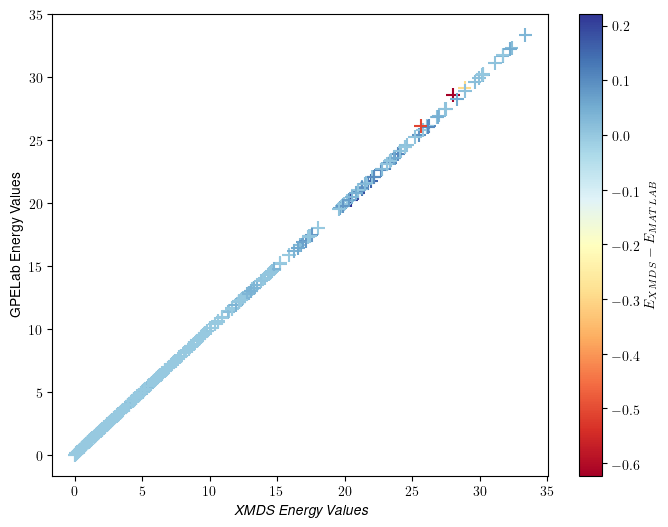
\includegraphics[width=\linewidth]{comparison-energy}
\caption{Error in density and energy}
\label{fig:dens_energy_error}
\end{figure}


\graphicspath{{"../figs/potentials/"}}
\begin{figure}[H]
    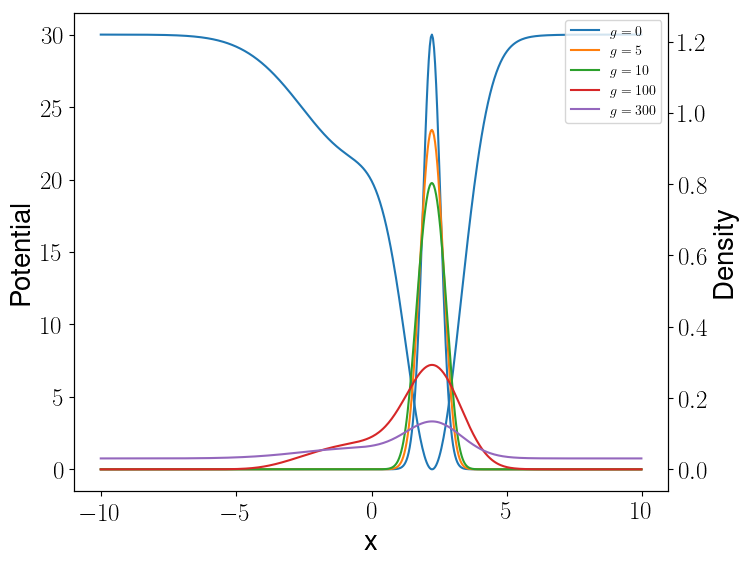
\includegraphics[width=\linewidth]{solutionswithinter}
    \caption{Density under Double Inverted Gaussian Potential with different interaction parameter.}
\label{fig:gaussian_pot_and_density}
\end{figure}

\subsubsection{Brief info about imaginary time evolution. (detailed in APPENDIX)}
%\subsubsection{XMDS framerwork and other programs.}
\subsubsection{Potential generation} \label{sec:potential_generation}

In potential generation, we built a modular structure such that the algorithms to generate potentials are independent from the restrictions forced by numerical techniques such as boundary conditions or scaling. A python class object responsible for handling this process. This class is constructed with suitable parameters such as "number of points", "width" etc. The generated potentials are sent to another method supplied by class. This method re-scales, and applies an envelope function to ensure that potential goes to numerical limit at boundaries which is given as,
\begin{equation}
\label{eq:potential_boundary_conditions}
\begin{split}
    V(x < x_l) = V_0 \\ 
    V(x > x_r) = V_0
\end{split}
\end{equation}

To handle these conditions, we define two envelope functions given by the following expressions, 

\begin{equation}
\label{eq:envelope_potential_lr}
    \text{Env}_{LR}(x) = [(1 + \tanh{(\beta(x + x_L))}) + (1 - \tanh{(\beta(x + x_R))})]/2
\end{equation}

\begin{equation}
\label{eq:envelope_potential_m}
    \text{Env}_{M}(x) = 1 - \text{Env}_{LR}(x)
\end{equation}

where $x_L$ and $x_R$ are bounds given in the Table~\eqref{tb:general_table} and the plot is given in Fig.~\ref{fig:envelope_and_random_withot_pros}.  

\graphicspath{{"../figs/potentials/"}}
\begin{figure}[H]
\centering
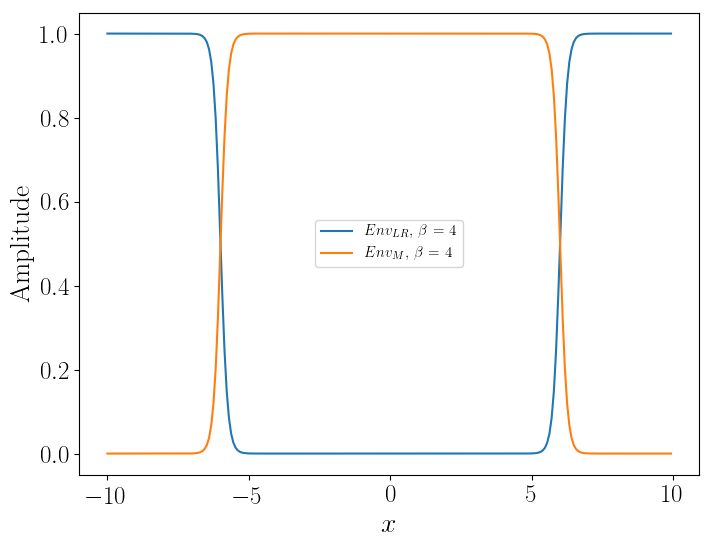
\includegraphics[width=.8\linewidth]{env}
\caption{Envelope Function}
\label{fig:envelope_and_random_withot_pros}
\end{figure}

As shown in Fig.~\ref{fig:envelope_and_random_withot_pros} $Env_{M}$ neutralizes the values while $x$ goes to boundaries and only the region in the middle survives. For $Env_{LR}$ the scenario is vice versa. Simultaneous application of these functions plus re-scaling brings the potential desired form shown in Fig.~\ref{fig:random_plus_envelope}


\graphicspath{{"../figs/potentials/"}}
\begin{figure}[H]
    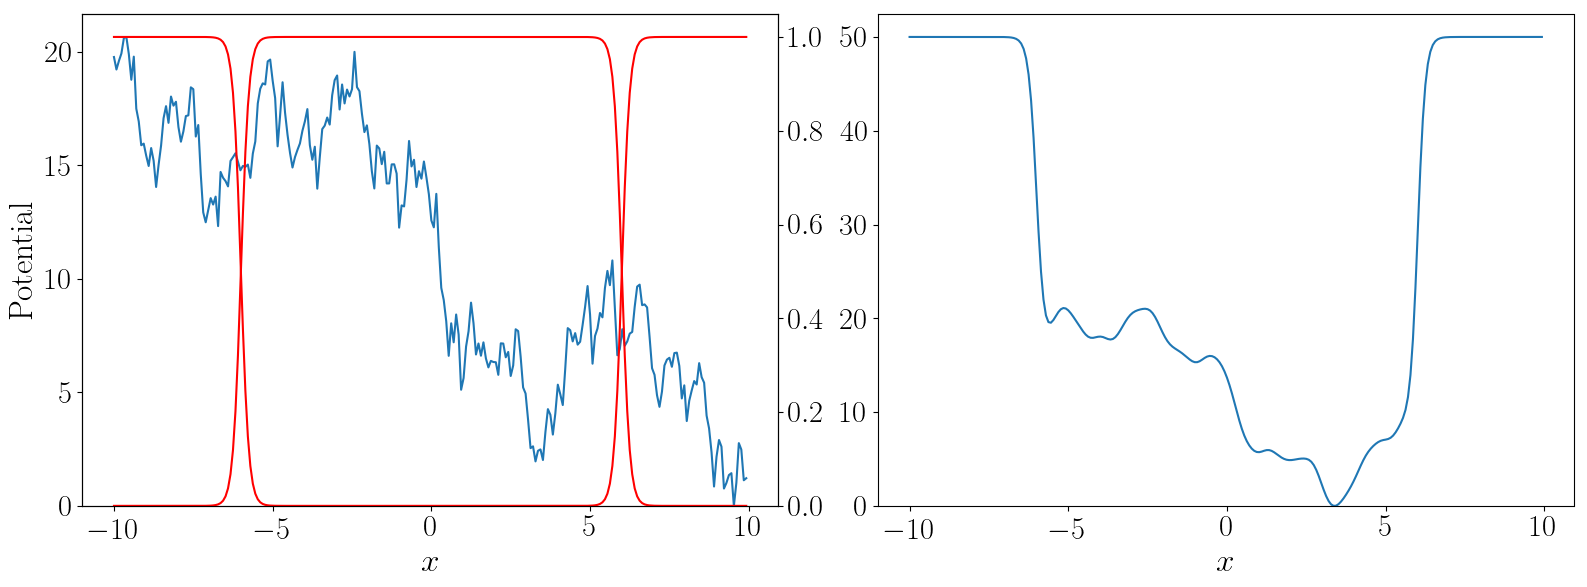
\includegraphics[width=\linewidth]{randombeforeafterproc}
\caption{Envelope functions are applied to a random potential. After that, a gaussian filter is applied for smoothness.}
\label{fig:random_plus_envelope}
\end{figure}





\subsubsection{Potential types (with analytic forms etc.)}

We use \textbf{six} different types of potential in our study. The first three potential which have analytic form given in Table~\ref{tb:general_table}. are 1D version of potentials studied in \cite{mills2017deep}. We implement two more random potential generator to study effect of generation process. The generation processes of the random potentials are described in Section~\ref{sec:random_potential_gen}.

\newcommand{\infinitewell}{$
V(x) = 
    \begin{cases}
       0 &\quad\text{if } x_l < x < x_r  \\
       \infty &\quad\text{if } \textit{otherwise} \\
    \end{cases}
$}

\newcommand{\harmonicpot}{$ V(x) =  \frac{1}{2}m \omega^2 (x - x_0) ^2 $}
\newcommand{\gaussianpot}{$V(x) = -A_1 \exp(\frac{(x - \mu_1)^2}{\sigma_1^2}) -A_2 \exp(\frac{(x - \mu_2)^2}{\sigma_2^2})$}
\newcommand{\randomexplation}{Summation of sines and cosines with random coefficients}
\newcommand{\envelopepotLR}{$\text{Env}_{LR}(x) = [(1 + \tanh{(\beta(x + x_L))}) + (1 - \tanh{(\beta(x + x_R))})]/2$}
\newcommand{\envelopepotM}{$\text{Env}_{M}(x) = 1 - \text{Env}_{LR}(x)$}
\newcommand{\randompotONE}{$V(x_{i+1}) = V(x_i) + [X\sim\mathcal{N}(\mu, \sigma)$]}



\begin{sidewaystable}
\begin{table}[H]
\centering
\caption{Potentials}
\label{tb:general_table}
\begin{tabular}{|l|l|l|l|l|l|} \hline
Potential                      & Analytic Form / Explanation         & Parameters           & Min   & Max  & Distribution \\ \hline
\multirow{3}{*}{Envelope}      & \multirow{2}{*}{\envelopepotLR}     & $x_L$                & -9    & 4.5  &              \\ 
                               & \multirow{2}{*}{\envelopepotM}      & $x_R$                & -4.5  & 9    &              \\
                               &                                     & $\beta$              & -4.5  & 9    &              \\ \hline
\multirow{3}{*}{Infinite Well} & \multirow{3}{*}{\infinitewell}      & $x_l$                & -9    & 4.5  &              \\ 
                               &                                     & $x_r$                & -4.5  & 9    &              \\
                               &                                     & $x_r - x_l$          & 1     & 8    &              \\ \hline
\multirow{2}{*}{Harmonic}      & \multirow{2}{*}{\harmonicpot}       & $\omega$             & 0.01  & 3    &              \\ 
                               &                                     & $x_0$                & -5    & 5    &              \\ \hline
\multirow{3}{*}{DI Gaussian}   & \multirow{3}{*}{\gaussianpot}       & $A_1, A_2$           & 1     & 10   &              \\ 
                               &                                     & $\mu_1, \mu_2$       & -5    & 5    &              \\
                               &                                     & $\sigma_1, \sigma_2$ & 0.5   & 4    &              \\ \hline
\multirow{2}{*}{Random\#1}     & \multirow{2}{*}{\randompotONE}      & $\mu$                & -4    & 4    &              \\ 
                               &                                     & $\sigma$             & 0.5   & 4    &              \\ \hline
\multirow{4}{*}{Random\#2}     & \multirow{4}{*}{\randomexplation}   & Number of Terms      & 1     & 100  &              \\ 
                               &                                     & $A_1, A_2$           & -4    & 4    &              \\
                               &                                     & $n_1, n_2$           & -6.30 & 6.30 &              \\
                               &                                     & $\sigma$             & 0.1   & 10   &              \\ \hline 
Random\#3                      & Substraction of two binary grid     & Scale Factor         & 8     & 8    &              \\ \hline

\end{tabular}
\end{table}
\end{sidewaystable}



\subsubsection{Random potential generations with different method. (Reason)}
\label{sec:random_potential_gen}

To be able to observe the effect of random potential generation to the results we use three different random potential generation algorithms. The first one is random walk with random step size such that the first value of the potential array is initialized with a random number. After that, another random number is added to this value to obtain the next element of the array and so on. The distribution of the random numbers is gaussian in this process. The resultant array is not guaranteed to be smooth. Gaussian filter is applied with a random sigma value to the potential array to make it smooth.    

\begin{algorithm}[H]
    \caption{RandomPotential1}\label{euclid}
    \begin{algorithmic}[1]
    \Procedure{RandomPotential1}{}
        \State $ Points = GaussianDistributedRandomPoints()$
        \State $Len = \textit{Length(Points)}$
        \State $Potential[0] = Points[0]$
        \For{$\text{i} = 0 \textbf{ to } Len - 1$}
        \State $Potential[i + 1] = Potential[i] + Points[i]$
        \EndFor
        \State $Potential = GaussianFilter(Potential, \sigma)$ 
    \EndProcedure
    \end{algorithmic}
\label{alg:random_potential_1}
\end{algorithm}

\graphicspath{{"../figs/potentials/"}}
\begin{figure}[H]
    \centering
        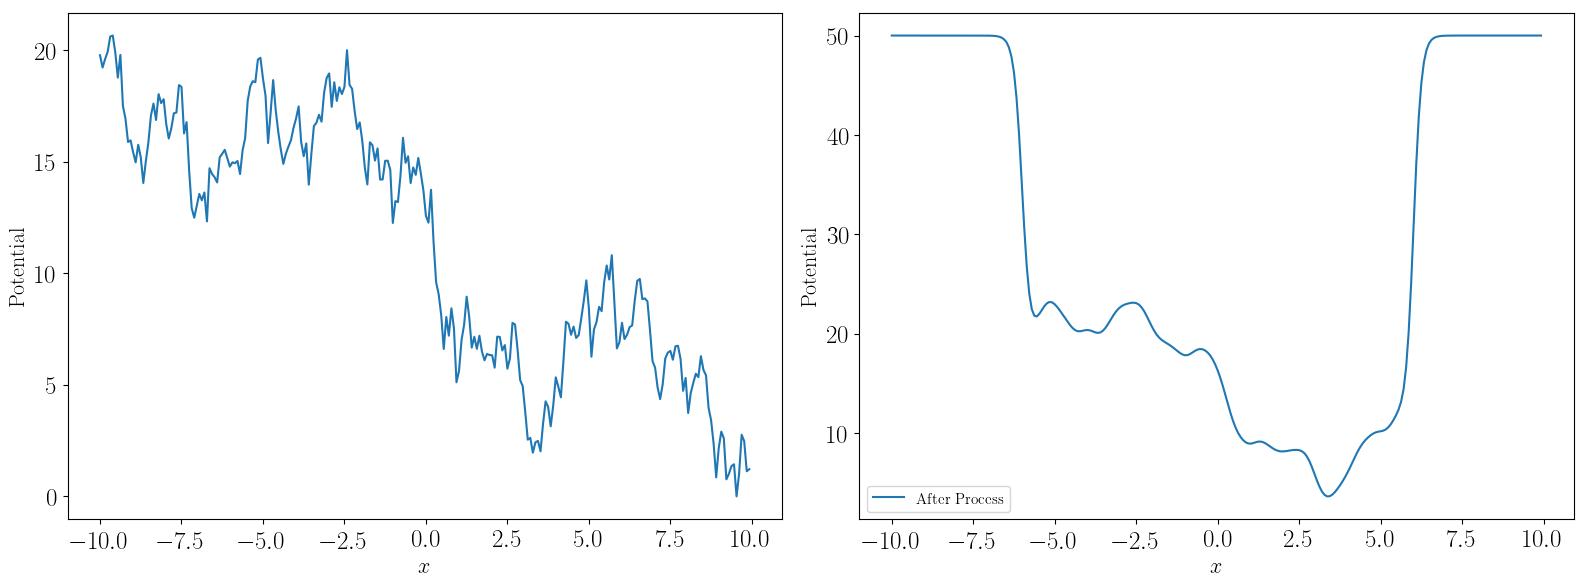
\includegraphics[width=\linewidth]{random-1-noprocandproc}
\caption{Random Potential 1 Before and After Process}
\label{fig:random1_before_after}
\end{figure}



The second one is summation of sines and cosines with random coefficients. Firstly, the number of terms are determined, after that each coefficient of the terms are assigned and summed iteratively.

\begin{algorithm}[H]
    \caption{RandomPotential2}\label{euclid}
    \begin{algorithmic}[1]
    \Procedure{RandomPotential2}{}
        \State $ Nterms = RandomInteger(1, 100)$
        \For{$\text{i} = 0 \textbf{ to } Nterms$}
        \State $A = GaussianDistributedRandomNumber()$
        \State $B = GaussianDistributedRandomNumber()$
        \State $n_1 = GaussianDistributedRandomNumber() * \sigma*\pi / width  $
        \State $n_2 = GaussianDistributedRandomNumber() * \sigma*\pi / width  $
        \State $Potential \mathrel{+}= A\sin(n_1 x) + B\cos(n_2 x)$
        \EndFor
        \State $Potential = GaussianFilter(Potential, \sigma)$ 
    \EndProcedure
    \end{algorithmic}
\label{alg:random_potential_1}
\end{algorithm}

\graphicspath{{"../figs/potentials/"}}
\begin{figure}[H]
    \centering
        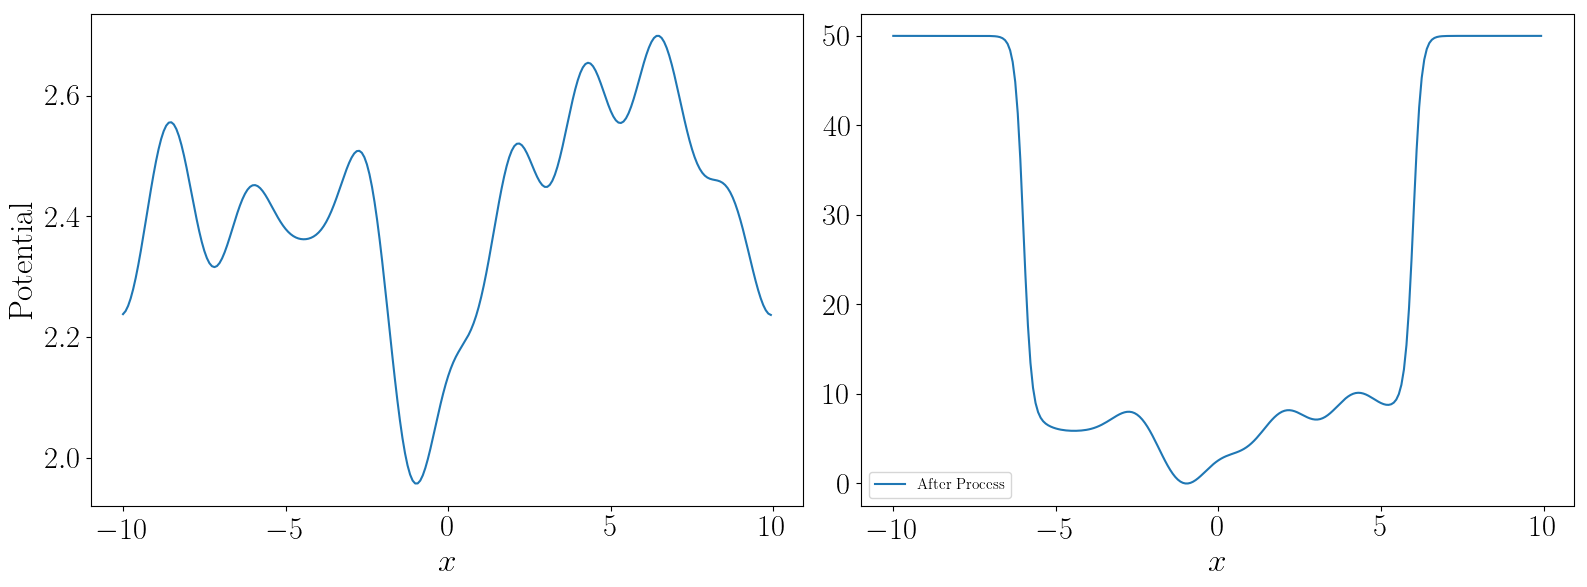
\includegraphics[width=\linewidth]{random-2-noprocandproc}
\caption{Random Potential 2 Before and After Process}
\label{fig:random2_before_after}
\end{figure}

The third one is one dimensional version of the algorithm described in \cite{mills2017deep} with slight modification. First a binary array of length $16$ is generated by assigning random ones or zeros. Then the array is upscaled to $128$ by repeating each element of the array $8$ times. After that, another binary array of length $8$ is generated with the same procedure and upscaled to $64$ by repeating elements. Left and right paddings of length $32$ is added to the second binary array to be able to do element wise substraction between two binary array. Then, the second array is substracted from the first one to obtain the potential in binary form. Finally, a gaussian filter is applied to make the potential smooth. 

\begin{algorithm}[H]
    \caption{RandomPotentia3}\label{euclid}
    \begin{algorithmic}[1]
    \Procedure{RandomPotential3}{}
        \State $ \textit{ScaleFactor} = 8$
        \For{$\text{i} = 0 \textbf{ to } \textit{NumberOfPoints/ScaleFactor}$}
        \State $BinaryGrid[i] = RandomInteger(0, 1)$
        \EndFor
        \State $BinaryGrid = RepeatElements(BinaryGrid, ScaleFactor)$
        \For{$\text{i} = 0 \textbf{ to } NumberOfPoints/(ScaleFactor * 2)$}
        \State $BinaryGrid2[i] = RandomInteger(0, 1)$
        \EndFor
        \State $BinaryGrid2 = RepeatElements(BinaryGrid, ScaleFactor)$
        \State $Padding = Zeros((Length(BinaryGrid) - Length(BinaryGrid2))/2)$
        \State $BinaryGrid2 = Concatanate(Padding, BinaryGrid2, Padding) $
        \State $Potential = BinaryGrid - BinaryGrid2$
        \State $Potential = GaussianFilter(Potential, \sigma)$ 
    \EndProcedure
    \end{algorithmic}
\label{alg:random_potential_1}
\end{algorithm}

\graphicspath{{"../figs/potentials/"}}
\begin{figure}[H]
    \centering
        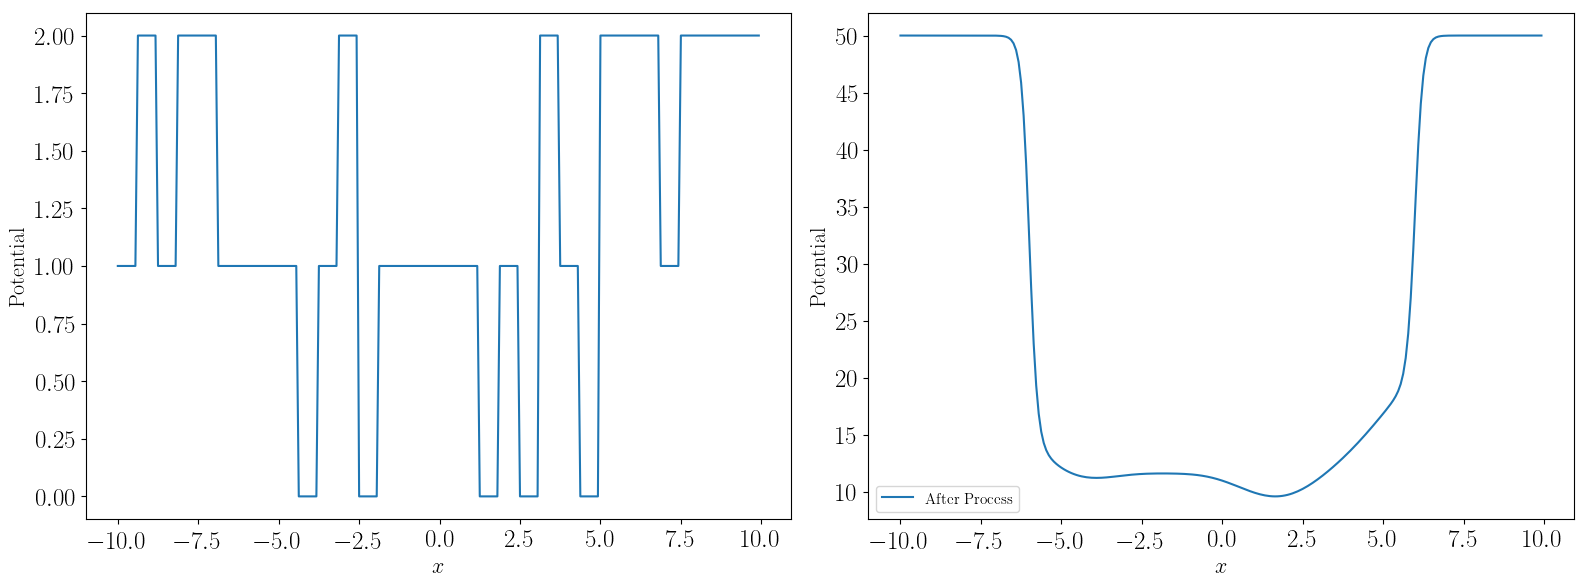
\includegraphics[width=\linewidth]{random-3-noprocandproc}
\caption{Random Potential 3 Before and After Process}
\label{fig:random3_before_after}
\end{figure}

\subsubsection{Density and Ground State Energy}

\graphicspath{{"../figs/potentials/"}}
\begin{figure}[H]
    \centering
    \begin{subfigure}[t]{0.45\textwidth}
        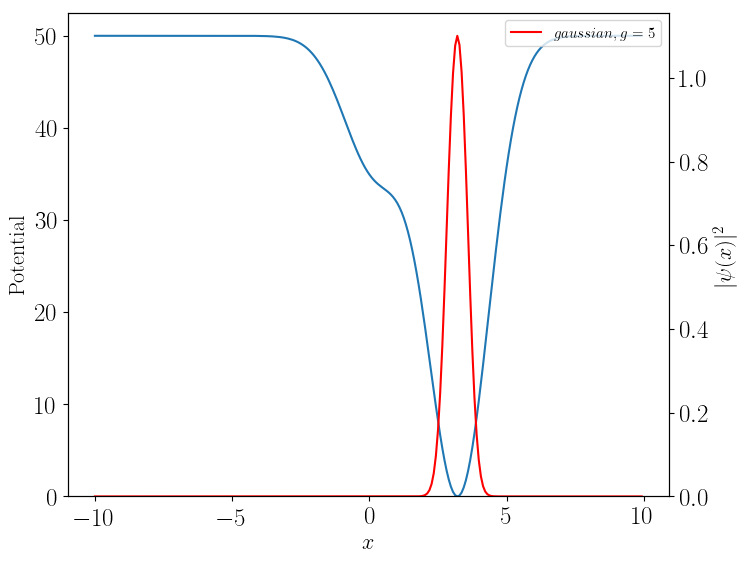
\includegraphics[width=\linewidth]{potvsdensity-gaussian}
    \end{subfigure}
    \begin{subfigure}[t]{0.45\textwidth}
        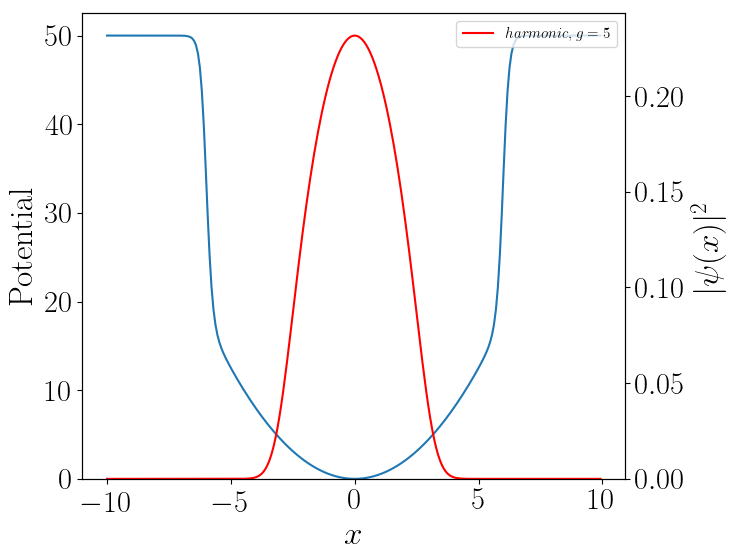
\includegraphics[width=\linewidth]{potvsdensity-harmonic}
    \end{subfigure}
    \begin{subfigure}[t]{0.45\textwidth}
        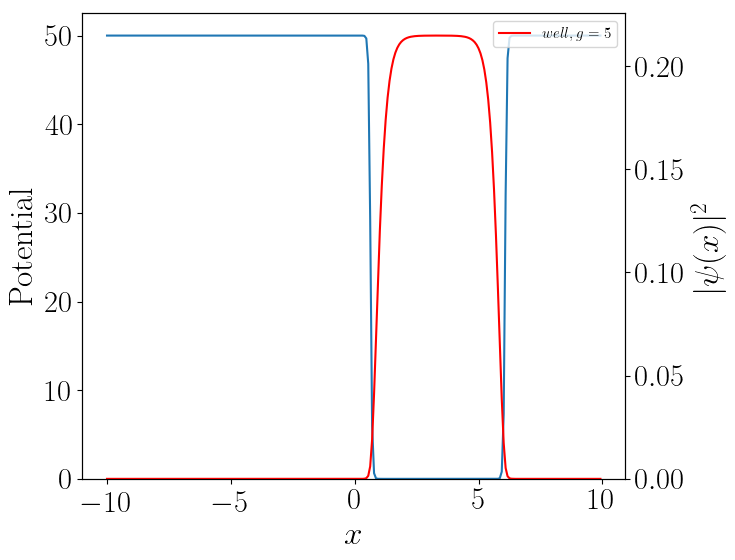
\includegraphics[width=\linewidth]{potvsdensity-well}
    \end{subfigure}
    \begin{subfigure}[t]{0.45\textwidth}
        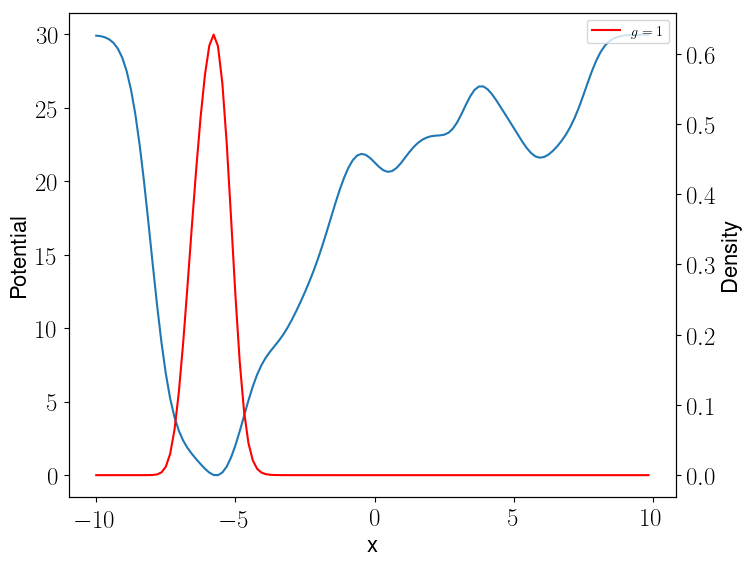
\includegraphics[width=\linewidth]{potvsdensity-random}
    \end{subfigure}
    \begin{subfigure}[t]{0.45\textwidth}
        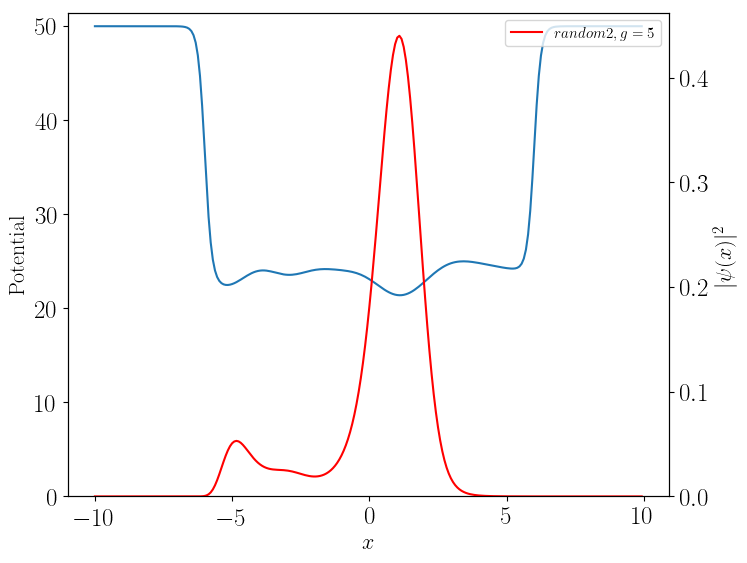
\includegraphics[width=\linewidth]{potvsdensity-random2}
    \end{subfigure}
    \begin{subfigure}[t]{0.45\textwidth}
        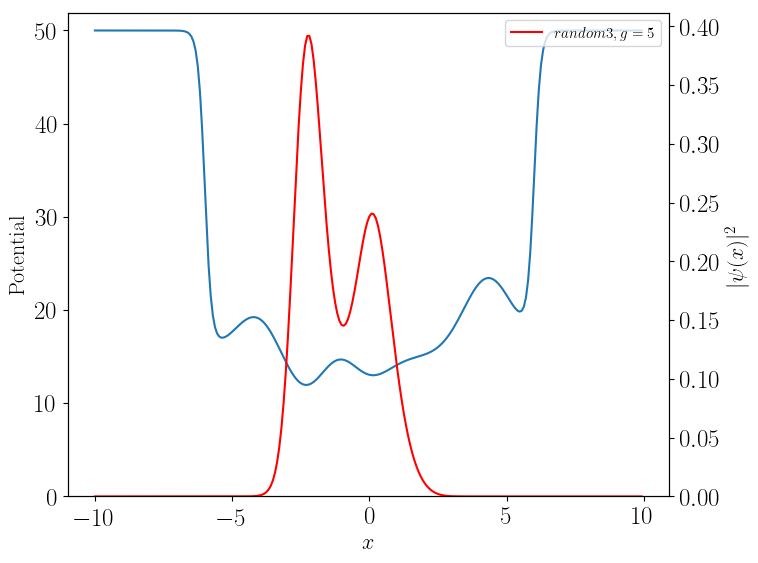
\includegraphics[width=\linewidth]{potvsdensity-random3}
    \end{subfigure}
\caption{Potentials and Corresponding Ground State Densities}
\label{fig:random3_before_after}
\end{figure}





\subsubsection{Boundaries. (Table)}
\subsubsection{Convergence (detailed in APPENDIX)}
\subsubsection{Dataset generation. (Total number of examples etc)}

\subsection{Dataset Features}
\subsubsection{Energy distribution}

%\graphicspath{{"../figs/dataresults/gaussian/"}}
%\begin{figure}[H]
%    \centering
%    \begin{subfigure}[t]{0.45\textwidth}
%		%\centering
%        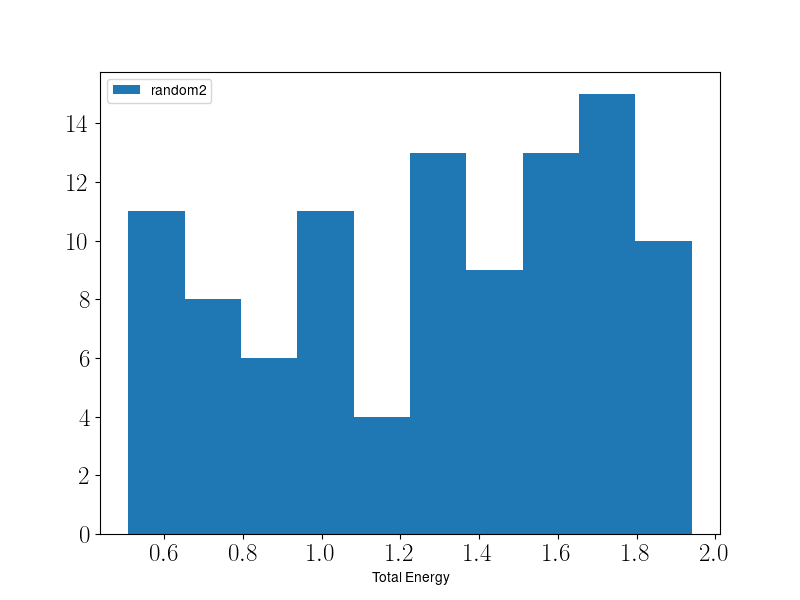
\includegraphics[width=\linewidth]{total}
%        \caption{g = 0}
%		
%    \end{subfigure}
%    \caption{Total energy distributions of the generated solution for different %interaction parameter values.}
%\label{fig:energy_dist}
%\end{figure}


\section{Machine Learning}
\subsection{Network architecture}
\noindent Architecture of the network.\\
    A general figure like in the ML\&SE article that describes the work done.\\
    Another figure about internals of the network such as number of layers, how interaction parameter is introduced to the network etc.\\
    Hyperparameters.\\
\subsection{Training}
\noindent    Detailed info about dataset (energy distribution etc).\\
    Indicate that if there is any method to increase the number of examples in low and high energy values.

\subsection{Results}

\section{Inverse Problem}

\clearpage
\section{Conclusion and Discussion}
\subsection{Conclusion}
\subsection{Discussion}
\subsection{Effects of random potential generation method}
\subsection{Are there problems in low and high energies compared to the mean}
\subsection{Inverse problem}


\clearpage

\clearpage
\bibliographystyle{ieeetr}
\bibliography{references}


\appendix
\section{APPENDIX A}
\label{ap:scale}

\textbf{Obtaining harmonic trap potential scaling from Eq.~\eqref{eq:GPE_dimensionless}}

\begin{equation}
\label{eq:GPESCALE_harmonic_potential_transform}
    V(x) \rightarrow V(\widetilde{x}) \rightarrow \widetilde{V}(\widetilde{x})
\end{equation}

\begin{equation}
\label{eq:GPESCALE_dimensionless_harmonic_potential}
    \widetilde{V}(x) \equiv \frac{V(x)}{\gamma E_0}
\end{equation}

\begin{equation}
\label{eq:GPESCALE_dimensionless_length}
    \widetilde{x} \equiv \frac{x}{\beta L} 
\end{equation}

\begin{equation}
\label{eq:GPESCALE_harmonic_potential}
    V(x) = \frac{1}{2}m\omega^2 (x-z_0)^2
\end{equation}

\begin{equation}
\label{eq:GPESCALE_harmonic_length_transform}
    V(\widetilde{x}) = \frac{1}{2}m\omega^2 \beta^2 L^2 (\widetilde{x}-\widetilde{z_0})^2
\end{equation}

\begin{equation}
\label{eq:GPESCALE_harmonic_energy_transform}
    \widetilde{V}(\widetilde{x}) = \frac{1}{2} m\omega^2 \frac{\beta^2 L^2}{\gamma E_0} (\widetilde{x}-\widetilde{z_0})^2  
\end{equation}

The coefficient of this equation must be dimensionless, therefore;

\begin{equation}
\label{eq:GPESCALE_harmonic_coeff}
    \frac{1}{2} m\omega^2 \frac{\beta^2 L^2}{\gamma E_0} = C
\end{equation}

Where $C$ is a positive constant. We know that $E_0 = \frac{\hbar^2}{2m}$ and the definition of $\alpha$ is given as,

\begin{equation}
\label{eq:GPESCALE_alpha}
    \frac{\hbar^2}{2m\gamma E_0} \frac{1}{\beta^2 L^2} = \alpha
\end{equation}
thus;

\begin{equation}
\label{eq:GPESCALE_gamma}
     \frac{1}{\gamma} = \alpha \beta^2 L^2
\end{equation}

if we plug Eq.~\eqref{eq:GPESCALE_gamma} in to Eq.~\eqref{eq:GPESCALE_harmonic_coeff}, then equation becomes,

\begin{equation}
\label{eq:GPESCALE_harmonic_coeff_2}
    \frac{m^2\omega^2}{\hbar^2} \alpha \beta^4 L^4 = C 
\end{equation} 

in the case of expressing same physical system, $m$ and $\omega$ must be constant. In that case $\alpha = C (\beta L)^{-4}$.\\


In this case, $\alpha$ becomes

$$ \alpha =  \frac{1}{2} \left(\frac{\hbar \omega}{\gamma E_0}\right)^2 $$

Conventionally, $\alpha$ is set to $1/2$, therefore;

$$ \hbar \omega = \gamma E_0 $$

$$ \beta L = \sqrt{\frac{\hbar}{m\omega}} $$ 

$ \beta L $ is generally defined as harmonic oscillator length $\ell$

$$ \ell = \sqrt{\frac{\hbar}{m\omega}} $$ 

$$ \widetilde{\mu} = \frac{\mu}{\hbar \omega} $$ 

$$ \widetilde{g} = \frac{g}{\hbar \omega \ell} $$

Finally, dimensionless GPE scaled for harmonic trapping potential can be written as,

$$\widetilde{\mu} \widetilde{\psi} = -\frac{1}{2}\frac{d^2\widetilde{\psi}}{d\widetilde{x}^2} + \frac{1}{2}\widetilde{x}^2\widetilde{\psi} + \widetilde{g}|\widetilde{\psi}|^2 \widetilde{\psi} $$


\end{document}
